\documentclass[a4paper, 12pt]{article}

\usepackage[utf8]{inputenc}
\usepackage[T1]{fontenc} 
\usepackage[english]{babel}

\usepackage[margin=3.0cm]{geometry}
\usepackage[margin=2cm,font={small,it}]{caption}

\usepackage{xcolor}
\usepackage{amsmath}
\usepackage{amsfonts}
\usepackage{amssymb}
\usepackage{amsthm}
\usepackage{graphicx}
\usepackage{float}
\usepackage{subcaption} %allows caption of subfigures

\usepackage{hyperref}
\usepackage[mode=buildnew]{standalone}% requires -shell-escape % or not lol
\usepackage{minted} % syntax highlighting
\definecolor{mygray}{gray}{0.95} % new color

\renewcommand{\thesection}{\Roman{section}}
\setminted[SQL]{
bgcolor=mygray,
frame=lines,
framesep=2mm,
breaklines, 
breakautoindent=true
}

\begin{document}
\title{Graph-based Knowledge Representation : Movie Database in Neo4j}
\author{Justine Sauvage, Victor Mercklé}
\maketitle

\section{Describe your dataset}
\subsection{}
Get the set of all distinct node labels.

\begin{minted}{SQL}
MATCH (n) RETURN DISTINCT labels(n);
\end{minted}

The command labels return the labels of n.

The command DISTINCT is used so that we returned each label only once.

Notice that if another label for node is allowed but do not appeared in the graph, it won't be returned by this query.

\subsection{}
Get the set of all distinct relationship types in the dataset.

\begin{minted}{SQL}
MATCH (n)-[r]-(m) RETURN DISTINCT type(r);
\end{minted}

The command type return the labels of r.

The command DISTINCT is used so that we returned each type only once.

\subsection{}
Get the set of all properties for different node labels and relationship types.

\begin{minted}{SQL}
MATCH (n)
WITH (labels(n))[0] as name,  keys(n) as kn
UNWIND kn as keyn
RETURN DISTINCT name,COLLECT(DISTINCT keyn) as properties
UNION
MATCH (n)-[r]-(m)
WITH type(r) as name, keys(r) as kr
UNWIND kr as keyr
RETURN DISTINCT name ,COLLECT(DISTINCT keyr) as properties;
\end{minted}

We make two queries to get the labels/types and properties of nodes as well as arrows. We then concatenate them with UNION.

For the first query we do : for each node in the graph, we get its label and list of properties. Then we break the list into rows (with the command unwind).

This allows us to then regroup for all label, all the properties that have been encountered with it in a single list. This is done with the command "COLLECT", to regroup all properties.

The command DISTINCT is used so that properties do not appears more than once in the same list.

The second query is similar to the first one.

\section{Adding more data}
\subsection{}
U1. Add Meryl Streep as a node.

U2. Add the movie The River Wild as a node .

U3. Add an ACTED\_IN relationship including Meryl’s role between the two.

U4. Add an ACTED\_IN relationship including the role between Kevin Bacon and The River Wild.

U5. For The Bridges of Madison County, add nodes corresponding to the movie, to its three main actors, and to its director, as well as ACTED\_IN/DIRECTED edges.

\begin{minted}{SQL}
MATCH (Kevin:ShowbizPerson),(Clint:ShowbizPerson)
WHERE Kevin.name="Kevin Bacon"
AND Clint.name="Clint Eastwood"
CREATE (Streep:ShowbizPerson {name:'Meryl Streep', born:1949})
CREATE (Annie:ShowbizPerson {name:'Annie Corley', born:1952})
CREATE (River:Movie {title:'The River Wild', released:1995, tagline:'Rafting expert Gail takes on a pair of armed killers while navigating a spectacularly violent river.'})
CREATE (Madison:Movie {title:'The Bridges of Madison County', released:1995, tagline:'Photographer Robert Kincaid (Clint Eastwood) wanders into the life of housewife Francesca Johnson (Meryl Streep) for four days in the 1960s.'})
CREATE (Streep)-[:ACTED_IN {roles:['Gail Hartman']}]->(River)
CREATE (Kevin)-[:ACTED_IN {roles:['Wade']}]->(River)
CREATE (Clint)-[:ACTED_IN {roles:['Robert Kincaid']}]->(Madison)
CREATE (Annie)-[:ACTED_IN {roles:['Carolyn Johnson']}]->(Madison)
CREATE (Streep)-[:ACTED_IN {roles:['Francesca Johnson']}]->(Madison)
CREATE (Clint)-[:DIRECTED]->(Madison);
\end{minted}

We apply the same thing that what is done in the given sql file.

Notice that we collected already existing nodes through matching.

\section{Querying simple patterns}
\subsection{}
Find all actors that directed a movie they also acted in.

Return actor and movie nodes.

\begin{minted}{SQL}
MATCH (n:ShowbizPerson)-[:ACTED_IN]->(m:Movie)<-[:DIRECTED]-(n)
RETURN n,m;
\end{minted}

We simply match the pattern to get the results.

\subsection{}
Find all reviewer pairs, one following the other and both reviewing the same movie.

Return the entire subgraphs.

\begin{minted}{SQL}
MATCH p=(m:Movie)<-[:REVIEWED]-(n1:MoviegoerPerson)-[:FOLLOWS]->
(n2)-[:REVIEWED]->(m)
RETURN p;
\end{minted}

Similarly, we can match the exact pattern.

\subsection{}
Find all reviewer pairs, such that one follows the other.

Return the two reviewers and a movie they may have reviewed both

\begin{minted}{SQL}
MATCH (n1:MoviegoerPerson)-[:FOLLOWS]->(n2:MoviegoerPerson)
OPTIONAL MATCH (n1)-[:REVIEWED]->(m1:Movie)
OPTIONAL MATCH (n2)-[:REVIEWED]->(m2:Movie)
RETURN [n1.name, n2.name], collect(COALESCE(m1.title, m2.title))[0];
\end{minted}

Interpretation : for each pair, we return a movie reviewed by at least one of the two reviewers. (they both may have reviewed the movie)

OPTIONAL MATCH will replace missing instances (for example m1) with NULL in case no instances exists that fits the pattern.

If n1 has not reviewed any movie, m1 will be NULL.

COALESCE(a, b) will return a if a is not NULL. Otherwise it will return b. This ensures that if n1 has not reviewed any movie, but n2 did, we can still assign them a movie. Then we simply collect the movies and only take the first one.

\subsection{}
Restrict the previous query so that the name of the followed reviewer is 12 characters long.

Try a different position for the where clause. Explain why this gives a different result.

\begin{minted}{SQL}
MATCH (n1:MoviegoerPerson)-[:FOLLOWS]->(n2:MoviegoerPerson)
OPTIONAL MATCH (n1)-[:REVIEWED]->(m1:Movie)
OPTIONAL MATCH (n2)-[:REVIEWED]->(m2:Movie)
RETURN [n1.name, n2.name], collect(COALESCE(m1.title, m2.title))[0];
\end{minted}

We use a optional match to replace missing part of the match by NULL

If WHERE is right after the first match, we only get one result because Angela Scope is the only followed reviewer with length 12

If the WHERE is placed after the first or second optional match, we get as many results as without any WHERE clause. Indeed, the WHERE applies to the optional match, and not the first one. Thus all reviewers are matched.

On the second optional match, the where will apply, but since it's an optional match, all the matched movie m2 will simply be NULL, and because of the coalesce command, we will always take the movie reviewed by n1.

\subsection{}
Find all pairs of actors where both acted in a movie together after 2005.

Return the actor names and movie node with every pair of actors occurring just once

\begin{minted}{SQL}
MATCH (n1:ShowbizPerson)-[:ACTED_IN]->(m:Movie) <-[:ACTED_IN]-(n2:ShowbizPerson)
WHERE m.released >= 2005
AND n1.name < n2.name
RETURN DISTINCT [n1.name,n2.name],collect(m)[0];
\end{minted}

We return unique pairs of actors that have acted in the same movie released after 2005.

We match two actors nodes that have both an arrow [ACTED\_IN] toward the same movie node.

The test "n2.name<n1.name" assures that for all pairs of actors (a,b) one will only get the pair (min(a,b),max(a,b)) where the order used is the one used by cypher on strings.

Then, we only show the distinct pairs by aggregating the movies names, thus removing the duplicates pairs. Then we only show the first movie node with [0]

\subsection{}
Extend Q5 to find all other movies in which the actors computed by Q5 also acted in.

\begin{minted}{SQL}
MATCH (n1:ShowbizPerson)-[:ACTED_IN]->
(m:Movie) <-[:ACTED_IN]-(n2:ShowbizPerson)
WHERE m.released >= 2005
AND n1.name < n2.name
with n1, n2
MATCH (n1)-[:ACTED_IN]-> (m1:Movie)
WHERE m1.released >= 2005
with n1, n2, collect(m1.title) as m1x
MATCH (n2)-[:ACTED_IN]-> (m2:Movie)
WHERE m2.released >= 2005
with n1, n2, m1x + collect(m2.title) as mx
unwind mx as mxs
with distinct n1, n2, mxs
RETURN DISTINCT [n1.name,n2.name], collect(mxs);
\end{minted}

Interpretation : For each unique pair of actors (that have acted in a movie together after 2005), we return all the movies they have done on their own or together.

Here we match n1 and n2 as before, and then we collect the titles of the movie of n1 in a list and we append to that list the movies' title of n2. Then we unwind this list to create a unique list of movies and this concludes the query.

\section{Querying complex patterns}
\subsection{}
Match all reviewers and the one they are following directly or via another, third reviewer.

\begin{minted}{SQL}
MATCH (r:MoviegoerPerson)-[:FOLLOWS]->(r2)
RETURN r as reviewer, r2 as followed
UNION
MATCH (r:MoviegoerPerson)-[:FOLLOWS]->(r1:MoviegoerPerson)-[:FOLLOWS]->(r2)
RETURN r as reviewer, r2 as followed;
\end{minted}

We join the two queries that return couples of people where :

a) for the first query : the first person in the each couple follow the other ;

b) for the second query : the first person in the couple follow the other via a third one.

\subsection{}
Count the number of paths of at most length 4

starting from Clint Eastwood ignoring edge direction.

\begin{minted}{SQL}
MATCH path = (n:ShowbizPerson)-[*1..4]-(m)
WHERE n.name="Clint Eastwood"
RETURN count(distinct path);
\end{minted}

The command "[*1..4]" will match paths of length 1 to 4 that start with n and end with  m.

The command count counts the numbers of path.

The command distinct make sure we won't count same path twice.

Result : 182

\subsection{}
Count the number of paths of at most length 10

starting from Clint Eastwood ignoring edge direction.

\begin{minted}{SQL}
MATCH path = (n:ShowbizPerson)-[*1..10]-(m)
WHERE n.name="Clint Eastwood"
RETURN count(distinct path);
\end{minted}

Result : 570642

\subsection{}
Count the number of paths of at most length 11

starting from Clint Eastwood ignoring edge direction.

\begin{minted}{SQL}
MATCH path = (n:ShowbizPerson)-[*1..11]-(m)
WHERE n.name="Clint Eastwood"
RETURN count(distinct path);
\end{minted}

Result : 2054494

\subsection{}
Count the number of nodes reachable

in at most 4 hops starting from Clint Eastwood ignoring edge direction.

\begin{minted}{SQL}
MATCH (n:ShowbizPerson)-[*1..4]-(m)
WHERE n.name="Clint Eastwood"
RETURN count(distinct m);
\end{minted}

The command "[*1..4]" will match paths of length 1 to 4 that start with n and end with  m.

The command count counts the numbers of path.

The command distinct makes sure we won't count same path twice.

Result : 48

\subsection{}
Count the number of nodes reachable

in at most 10 hops starting from Clint Eastwood ignoring edge direction.

\begin{minted}{SQL}
MATCH (n)-[*1..10]-(m)
WHERE n.name="Clint Eastwood"
RETURN count(distinct m);
\end{minted}

Result : 175

\subsection{}
Count the number of nodes reachable

in at most 11 hops starting from Clint Eastwood ignoring edge direction.

\begin{minted}{SQL}
MATCH (n)-[*1..11]-(m)
WHERE n.name="Clint Eastwood"
RETURN count(distinct m);
\end{minted}

Result : 175

\section{Aggregate queries}
\subsection{}
Determine the average age of the Apollo 13 cast at the time of the movie’s release

\begin{minted}{SQL}
MATCH (n:ShowbizPerson)-[:ACTED_IN]-> (m:Movie)
WHERE m.title = "Apollo 13"
RETURN avg(m.released-n.born);
\end{minted}

The age for each actors when the movie was released is computed by m.released-n.born where n.born is the actor's birth year and m.released the date the movie was released.

The command avg compute the average of all rows.

\subsection{}
Find the movies with the top-10 oldest cast at the time of the movie’s release

Return movie and average age rounded to two decimal ordered by descending age

\begin{minted}{SQL}
MATCH (n:ShowbizPerson)-[:ACTED_IN]-> (m:Movie)
RETURN m,round(100*avg(m.released-n.born))/100 as mean
ORDER BY mean DESC
LIMIT 10;
\end{minted}

The command "order by ... desc" returns the result sorted in decreasing order.

The command LIMIT 10 return the first 10 results.

\subsection{}
Find average age of youngest actors in movie casts at time of release

\begin{minted}{SQL}
MATCH (n:ShowbizPerson)-[:ACTED_IN]-> (m:Movie)
WITH m,min(m.released-n.born) as mage
RETURN avg(mage);
\end{minted}

Interpretation : returns the average of all movies' youngest actor's age.

Using the command "WITH", for each movie, we only keep the minimum age of the cast.

Hence the average of age is the average age of the youngest actor of all movies.

\subsection{}
Return for each movie the name of the youngest actor, order by movie title and actor name.

\begin{minted}{SQL}
MATCH (n:ShowbizPerson)-[:ACTED_IN]-> (m:Movie)
WITH m.title as title, max(n.born) as maxx
MATCH (n:ShowbizPerson)-[:ACTED_IN]-> (m:Movie)
WHERE m.title = title AND n.born = maxx
return m.title, n.name
order by m.title, n.name;
\end{minted}

First we get the youngest actor (highest born year) for each movie.

Then we get the movie title and the youngest actor name associated with the birth-date computed in the first MATCH.

\subsection{}
Find ACTED\_IN subgraph of the movie with the youngest cast at the time of the movie’s release

\begin{minted}{SQL}
MATCH (n:ShowbizPerson)-[:ACTED_IN]-> (m:Movie)
WITH m.title as title, avg(m.released - n.born) as age
WITH min(age) as avgage
MATCH (n:ShowbizPerson)-[:ACTED_IN]-> (m:Movie)
WITH m, avgage, avg(m.released - n.born) as age
WHERE age = avgage
MATCH p= (a)-[:ACTED_IN]-> (m1:Movie)
WHERE m1.title = m.title
return p;
\end{minted}

We first compute the age of the youngest cast, then we match the movie which has the youngest cast. Then we simply match the path from an actor to this movie and return the named paths, this defines the ACTED\_IN subgraph.

\subsection{}
Determine the movie with youngest and movie with oldest cast and their age difference rounded to two decimals.

\begin{minted}{SQL}
MATCH (n:ShowbizPerson)-[:ACTED_IN]-> (m:Movie)
WITH m.title as oldest, avg(m.released - n.born) as age
WITH oldest, max(age) as maxage
MATCH (n:ShowbizPerson)-[:ACTED_IN]-> (m:Movie)
WITH oldest, m as youngest,
round((maxage - avg(m.released - n.born))*100)/100 as age
ORDER BY age DESC LIMIT 1
return oldest, youngest.title as youngest, age as age_difference;
\end{minted}

We first retrieve the maximum average age of a movie's cast then we again list movies with their average cast age subtracted by the maximum.

The movie with the youngest cast is the one associated with the biggest difference so we simply sort the results and take the first result.

This gives us the age difference between the youngest and oldest cast.

\section{Adjacency list and distribution}
\subsection{}
Return the whole graph as a simple adjacency list of vertex ids ordered in descending order.

\begin{minted}{SQL}
MATCH (a)-[e]->(b)
with id(a) as ida, id(b) as idb
order by ida DESC, idb DESC
return ida, collect(idb);
\end{minted}

We simply collect all the IDs.

\subsection{}
Return the out degree distribution ordered by ascending degree.

\begin{minted}{SQL}
MATCH (k)
WITH k, size((k)-->()) as degree
order by degree ASC
return degree;
\end{minted}

Here we have to use size in the WITH to catch vertices with 0 out degree.

\subsection{}
Return degree distribution ordered by ascending degree.

\begin{minted}{SQL}
MATCH (k)
WITH k, size((k)--()) as degree
order by degree ASC
return degree;
\end{minted}

Simple modification from Q2 to not take into account directionality of arrows.

\subsection{}
Return edge types with corresponding number of instances ordered by descending order.

\begin{minted}{SQL}
MATCH p = (a)-[e]->(b)
with type(e) as edge_type, count(p) as number_instances
order by number_instances DESC
return edge_type, number_instances;
\end{minted}

We simply count how many instances we have of each edge type.



\section{Measuring the running time of queries}
\begin{figure}
\centering
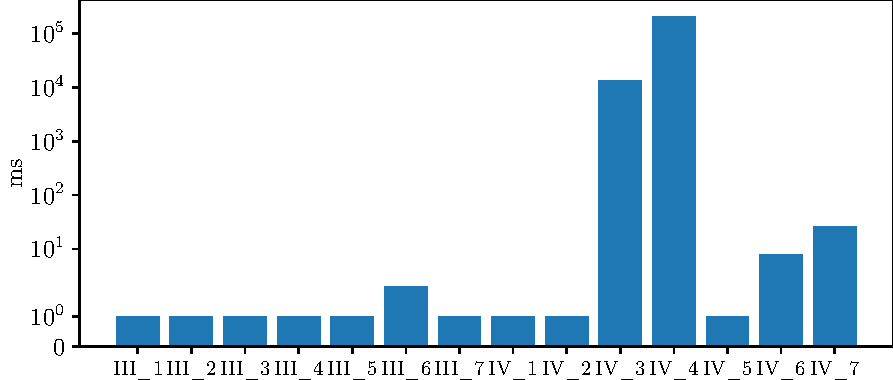
\includegraphics[scale=0.8]{graphtime}
\caption{Execution time of queries from III and IV sections}
	\label{topkek}
\end{figure}

In the barplot \ref{topkek}, we can see that all the queries in section III have a negligible execution time (<1ms). Only queries in section IV that deals with paths of certain length takes longer.

The two bars we can actually see are the time it takes to count all paths of length up to 10, and up to 11. There are 570642 paths of length<=10 and 2 054 494 of length<=11. The exponential amount paths is reflected in the exponential execution time. In figure \ref{topkek2} we ran the query with a finer range of length of paths. The plot is on a logarithmic scale and we can see it is somewhat linear and thus exponential in reality.

\begin{figure}
\centering
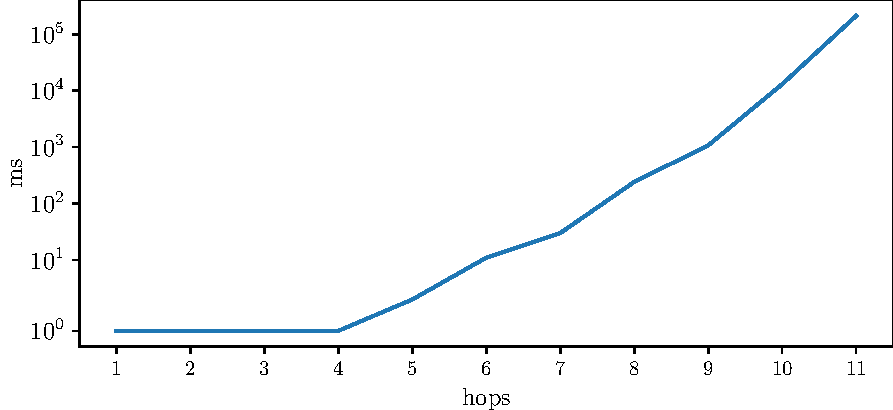
\includegraphics[scale=0.8]{graphtime2}
	\caption{Time taken to count the number of paths of various length}
	\label{topkek2}
\end{figure}

\begin{figure}
\centering
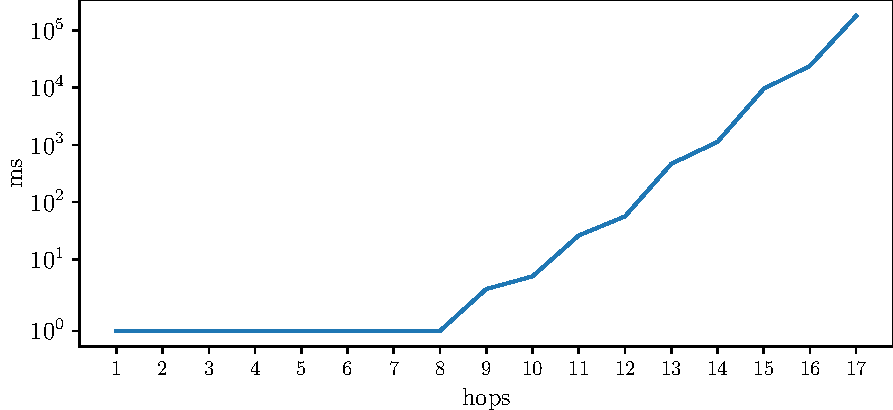
\includegraphics[scale=0.8]{graphtime4}
	\caption{Path counted per millisecond as the number of possible hops increases}
	\label{topkek3}
\end{figure}

Queries IV-7 only counts the number of reachable nodes in 11 hops. This query has been optimized as it takes only 26ms. It does not need to iterate through every path possible. However, in graph \ref{topkek3} we measured the execution time for a wider range of possible hops. We can see it is also of exponential complexity.



\end{document}
